\documentclass[addpoints,12pt]{exam}
\usepackage{amsmath, amssymb}
\linespread{1.1}
\usepackage{graphicx}
%\boxedpoints
%\pointsinmargin



\newcommand{\p}{\mathbb{P}}
\newcommand{\expect}{\mathbb{E}}
\newcommand{\var}{\mathbb{V}}
\newcommand{\cov}{Cov}
\newcommand{\cprob}{\rightarrow_{p}}
\newcommand{\cas}{\rightarrow_{as}}
\newcommand{\clp}{\rightarrow_{L^p}}
\newcommand{\clone}{\rightarrow_{L^1}}
\newcommand{\cltwo}{\rightarrow_{L^2}}
\newcommand{\cd}{\rightarrow_{d}}
\newcommand{\cv}{\Rightarrow_{v}}
\newcommand{\dec}{\downarrow}
\newcommand{\inc}{\uparrow}
\newcommand{\plim}{\hbox{plim}_{n\rightarrow \infty}}
\newcommand{\limn}{\lim_{n \rightarrow \infty}}
\newcommand{\fil}{(\mathcal{F}_n)_{n=0}^{\infty}}
\newcommand{\xn}{(X_n)_{n=0}^{\infty}}
\newcommand{\hn}{(H_n)_{n=0}^{\infty}}
\DeclareMathOperator*{\argmax}{arg\,max}
\DeclareMathOperator*{\argmin}{arg\,min}
\newcommand{\norm}[1]{\left|\left|#1\right|\right|}
\newcommand{\inprod}[1]{\left\langle#1\right\rangle}
\newcommand{\slfrac}[2]{\left.#1\right/#2}

%\printanswers
%\noprintanswers


\pagestyle{headandfoot}
\runningheadrule
\runningheader{Econ 103}
              {Final Exam, Page \thepage\ of \numpages}
              {December 12, 2012}

\runningfooter{Name: \rule{5cm}{0.4pt}}{}{Student ID \#: \rule{5cm}{0.4pt}}



%%%%%%%%%%%%%%%%%%%%%%%%%%%%%%%%%%%%%%%%%%%%%%%%%%%%%%%%%%%%%%%
\begin{document}

\begin{center}
\large
\sc{Final Examination\\ \normalsize Econ 103, Statistics for Economists \\ \vspace{0.5em} December 12, 2012}

\vspace{1em}

\normalsize
\fbox{\begin{minipage}{0.5\textwidth}
\textbf{You will have 120 minutes to complete this exam.
Graphing calculators, notes, and textbooks are not permitted. }\end{minipage}}


\end{center}
%%%%%%%%%%%%%%%%%%%%%%%%%%%%%%%%%%%%%%%%%%%%%%%%%%%%%%%%%%%%%%%

\vspace{2em}
\begin{center}
  \fbox{\fbox{\parbox{5.5in}{\centering
        I pledge that, in taking and preparing for this exam, I have abided by the University of Pennsylvania's Code of Academic Integrity. I am aware that any violations of the code will result in a failing grade for this course.}}}
\end{center}
\vspace{0.2in}
\makebox[\textwidth]{Name:\enspace\hrulefill}

\vspace{0.2in}
\noindent \makebox[\textwidth]{Student ID \#:\enspace\hrulefill}

\vspace{0.3in}
\noindent\makebox[\textwidth]{Signature:\enspace\hrulefill}

%\rule{1cm}{0.4pt}
\vspace{3em}

\begin{center}
  \gradetable[h][questions]
\end{center}

\vspace{3em}

\paragraph{Instructions:} Answer all questions in the space provided. Should you run out of space, continue on the back of the page. Show your work for full credit but be aware that writing down irrelevant information will not gain you points. Be sure to sign the academic integrity statement above and to write your name and student ID number on \emph{each page} in the space provided. Make sure that you have all pages of the exam before starting.

%%%%%%%%%%%%%%%%%%%%%%%%%%%%%%%%%%%%%%%%%%%%%%%%%%%%%%%%%%%%%%%
\newpage
\begin{questions}


\question[10] In an effort to reduce traffic fatalities, local authorities installed traffic cameras in particularly accident-prone locations in west London in 1992. In the preceding three years, there were 62 fatal accidents in these locations. In the three years following the introduction of the cameras, there were only 19 fatal accidents. Based on this evidence, local authorities concluded that traffic cameras reduce fatalities. Traffic cameras have since been installed in the whole of London. Using the information provided in this question \emph{only}, do we have good evidence that traffic cameras reduce the frequency of fatal accidents? Explain why or why not.
	\begin{solution}[2.8in]
	 No: this is an example of regression to the mean (the regression fallacy). The sites in question were chosen because they had unusually high fatalities. In any given period, the intersections with the greatest number of fatalities are likely to be intrinsically dangerous \emph{and} to have suffered a spell of ``bad luck.'' This is because fatalities are not perfectly correlated over time. Even if we had \emph{not} installed cameras, we would expect fatalities to be lower on average in the second period at those intersections that had unusually high numbers of fatalities in the first period. Students may also mention that we didn't discuss normalizing for volume of traffic.
	\end{solution}

\question[10] Of women who undergo regular mammograms, two percent have breast cancer. If a woman has breast cancer, there is a 90\% chance that her mammogram will come back positive. If she does \emph{not} have breast cancer there is a 10\% chance that her mammogram will come back positive. Given that a woman's mammogram has come back positive, what is the probability that she has breast cancer? 
	\begin{solution}[2.8in]
		 Let $B$ be the event that a given woman has breast cancer and $M$ be the event that her mammogram comes back positive. By Bayes' Rule,
		 		$$\p(B|M) = \frac{\p(M|B)\p(B)}{\p(M)}$$
	By the law of total probability, 
		 			\begin{eqnarray*}
		 			\p(M) &=& \p(M|B)\p(B) + \p(M|B^c)\p(B^c)\\
		 				&=& 0.9 \times 0.02 + 0.1 \times 0.98  = 0.018 + 0.098 = 0.116
		 			\end{eqnarray*}
		 	Hence,
		 		$$\p(B|M) = \frac{0.9 \times 0.02}{0.116} = \frac{0.018}{0.116} \approx 0.16$$
	\end{solution}


\question[15] Explain the difference between $\mu$, $\bar{X}_n$ and $\bar{x}$ using the concepts and terminology we have studied in this course. 
	\begin{solution}[3in]
		We use the symbol $\mu$ to denote the population mean. This a \emph{parameter}, in other words an unknown constant. Both of the remaining quantities are called the sample mean, but there is an important distinction between then. Whereas $\bar{X}_n$ is an \emph{estimator}, $\bar{x}$ is an \emph{estimate}. Under random sampling, $\bar{X}_n$ is a random variable: since the sample is random, the estimator is random. In contrast, $\bar{x}$ is a constant number, obtained by calculating the sample mean of the data (realizations) that we observed for in a \emph{particular sample}. In other words, $\bar{X}_n$ denotes \emph{process} of taking a random sample and computing the mean of that sample, whereas $\bar{x}$ denotes the \emph{result} of this process.
	\end{solution}

\question Let $X$ be a Uniform$(0,1)$ random variable.
	\begin{parts}
		\part[5] Write down the probability density function (pdf) and support of $X$.
			\begin{solution}[0.6in]
				$f(x) = 1$ for $x\in (0,1)$, zero otherwise.
			\end{solution}
		\part[5] Calculate the cumulative distribution function (cdf) of $X$.
			\begin{solution}[1.1in]
				$$F(x_0) = \int_{-\infty}^{x_0} f(x) \; dx = \int_{0}^{x_0}1 \; dx = \left. x\right|_0^{x_0} = x_0$$
			\end{solution}
		\part[5] Calculate $\expect[X]$
			\begin{solution}[1.1in]
				$$\expect[X] = \int_{-\infty}^{\infty} xf(x)\; dx = \int_0^1 x\; dx = \left. \frac{x^2}{2} \right|_0^1 = 1/2$$
			\end{solution}
		\part[5] Calculate $\expect[X^2]$
			\begin{solution}[1.1in]
				$$\expect[X^2] = \int_{-\infty}^{\infty} x^2 f(x) \; dx = \int_0^1 x^2 \; dx = \left. \frac{x^3}{3}\right|_0^1 = 1/3$$
			\end{solution}
		\part[5] Using the shortcut formula, calculate $Var(X)$.
			\begin{solution}[1in]
				$$Var(X) = \expect[X^2] - \expect[X]^2 = 1/3 - (1/2)^2 = 1/3 - 1/4 = (4-3)/12 = 1/12$$
			\end{solution}
	\end{parts}


\question[15] About as many boys as girls are born in hospitals. Many babies are born every week at City General. In Cornwall, a country town, there is a small hospital where only a few babies are born every week. A \emph{normal week} is one where between 45\% and 55\% of the babies are female. An \emph{unusual week} is one where more than 55\% are girls, or more than 55\% are boys. Do unusual weeks occur more often at City General or Cornwall? Explain your answer using what you learned about sampling distributions in this course.
	\begin{solution}[2.5in]
		Unusual weeks are more common at Cornwall because the variance of the sampling distribution of a sample proportion is lower the larger the sample size: $Var(\widehat{p}) = p(1-p)/n$. The idea here is that $p$ is the same at both hospitals, but $n$ is larger at City General. Thus, there will be more sampling variability, and consequently more unusual weeks, at Cornwall. Another way to answer this would be to appeal to the law of large numbers.
	\end{solution}
	
	
\question This question concerns the quantity $\tilde{p}$ used to construct the ``refined'' confidence interval for a population proportion that I introduced in class. Recall that $\tilde{p} = (n\widehat{p} +2)/(n+4)$, where $\widehat{p} = \left(\sum_{i=1}^n X_i\right)/n$ and $X_1, \hdots, X_n \sim \mbox{iid Bernoulli}(p)$.
	\begin{parts}
		\part[5] Is $\tilde{p}$ an unbiased estimator of $p$? If so, prove it. If not, calculate its bias.
			\begin{solution}[2.3in]
				\begin{eqnarray*}
					\expect[\tilde{p}] - p &=& \expect\left[ \frac{n\widehat{p}+2}{n+4} \right] - p =\frac{n\expect[\widehat{p}] + 2}{n+4} - p = \frac{np + 2 - p(n+4)}{n+4} =  \frac{2 - 4p}{n+4}
				\end{eqnarray*}
				Hence the bias depends on $2-4p$. If $p=1/2$, then $2-4p=0$ so $\tilde{p}$ is unbiased. For all other values of $p$, it is biased. When $p>1/2$, we have $2-4p<0$, so the bias is negative. When $p<1/2$, we have $2-4p>0$ so the bias is positive.
			\end{solution}	
		\part[5] Which has a higher variance: $\widehat{p}$ or $\tilde{p}$? Prove your answer.
			\begin{solution}[3in]
				To begin, we know that $Var(\widehat{p}) = p(1-p)/n$. Now,
					\begin{eqnarray*}
						Var(\tilde{p}) &=& Var\left( \frac{n\widehat{p} + 2}{n+4}\right)= \left(\frac{n}{n+4}\right)^2 Var(\widehat{p})  = \left(\frac{n}{n+4}\right)^2 \left(\frac{p(1-p)}{n}\right)\\
						&=& p(1-p)\left[ \frac{n}{(n+4)^2}\right]
					\end{eqnarray*}
					So it suffices to compare $1/n$ against $n/[(n+4)^2]$. We have:
					\begin{eqnarray*}
						\frac{n}{(n+4)^2} = \frac{n}{n^2 + 8n + 16} = \frac{1}{n + 8 + 16/n}
					\end{eqnarray*}
					Since $n < (n + 8 + 16/n)$, it follows that $1/(n + 8 + 16/n) < 1/n$. Therefore, $\tilde{p}$ has a lower variance than $\widehat{p}$. The difference is when $n$ is relatively small.
			\end{solution}
		\part[5] Using your answers to (a) and (b), calculate the mean-squared error of $\tilde{p}$. Is $\tilde{p}$ a consistent estimator of $p$? Prove your answer.
			\begin{solution}[2in]
			Combining (a) and (b),
				\begin{eqnarray*}
					MSE(\tilde{p}) = \left(\frac{2-4p}{n+4}\right)^2 + \left[\frac{np(1-p)}{(n+4)^2}\right] \rightarrow 0
				\end{eqnarray*}
				Hence, $\tilde{p}$ is a consistent estimator of $p$. 
			\end{solution}
	\end{parts}


\question Suppose that $X_1, \hdots, X_n \sim \mbox{iid }N(\mu, \sigma^2)$. Let $\bar{X}_n$ be the sample mean and $S^2$ be the sample variance. Except in part (d), you do not need to provide any justification for your answers.
	\begin{parts}
		\part[5] What is the sampling distribution of $\sqrt{n}(\bar{X}_n-\mu)/\sigma$? 
			\begin{solution}[0.5in]
				$N(0,1)$
			\end{solution}
		\part[5] What is the sampling distribution of $\sqrt{n}(\bar{X}_n-\mu)/S$?
			\begin{solution}[0.5in]
				$t(n-1)$
			\end{solution}
		\part[5] What is the sampling distribution of $(n-1)S^2/\sigma^2$?
			\begin{solution}[0.5in]
				$\chi^2(n-1)$
			\end{solution}
		\part[10] Using your answer to part (c), derive a $100\times (1-\alpha)$ confidence interval for the variance of a normal population based on a random sample of $n$ observations. Express the interval in terms of the appropriate R commands.
			\begin{solution}[3in]
				Define:
					\begin{eqnarray*}
					a &=& \texttt{qchisq}(\alpha/2, \texttt{df} = \texttt{n - 1})\\
					 b &=& \texttt{qchisq}(1-\alpha/2, \texttt{df} = \texttt{n - 1})
					 \end{eqnarray*}
			Then, by (c)
				\begin{eqnarray*}
				\p\left( a \leq \frac{(n-1)S^2}{\sigma^2}\leq b\right) &=& 1-\alpha \\
				\p\left( \frac{a}{(n-1)S^2} \leq \frac{1}{\sigma^2}\leq \frac{b}{(n-1)S^2} \right) &=& 1-\alpha \\				
				\p\left( \frac{(n-1)S^2}{b} \leq \sigma^2\leq \frac{(n-1)S^2}{a} \right) &=& 1-\alpha \\					
				\end{eqnarray*}
				Therefore, the desired confidence interval is
					$$\left[\frac{(n-1)S^2}{\texttt{qchisq}(1-\alpha/2, \texttt{df = } n-1)}, \frac{(n-1)S^2}{\texttt{qchisq}(\alpha/2, \texttt{df = } n-1)}\right]$$
			\end{solution}
	\end{parts}
	
	
	
\question Suppose that $X_1, \hdots, X_n \sim \mbox{iid Bernoulli}(p)$ and define $\widehat{p} = \sum_{i=1}^n X_i/n$.
	\begin{parts}
		\part[5] Calculate the standard deviation of the sampling distribution of $\widehat{p}$.
			\begin{solution}[1in]
				$$Var(\widehat{p}) = \frac{1}{n^2}\sum_{i=1}^n Var(X_i) = p(1-p)/n$$ 
				Hence, $SD(\widehat{p})=\sqrt{p(1-p)/n}$.
			\end{solution}
		\part[5] There is a technical term for the standard deviation of a sampling distribution. What is it?
			\begin{solution}[0.5in]
				Standard error (SE).
			\end{solution}
		\part[5] What value of $p$ maximizes the standard deviation of the sampling distribution of $\widehat{p}$? What is the maximized standard deviation? Be sure to check the second order condition.
			\begin{solution}[1.75in]
				It suffices to maximize the function $p(1-p) = p-p^2$. The FOC is $1-2p=0$ so that $p^*=1/2$. The second derivative of this function is $-2$ for all $p$, so we have a global maximum. The maximized standard deviation is $\sqrt{(1/2)^2/n} = (1/2)/\sqrt{n} = 1/(2\sqrt{n})$.
			\end{solution}
		\part[5] Sarah is a graduate student in the political science department and is preparing to carry out a poll designed to estimate the proportion of college students who support gay marriage. Sarah plans to construct a 95\% confidence interval based on her results and wants to gather enough data so that the margin of error of her poll is no more than 4\%. Based on your answer to part (c) and the \emph{textbook confidence interval} for a population proportion, what is the smallest sample size that Sarah should consider using in her poll?
			\begin{solution}[3in]
				The margin of error for a textbook 95\% confidence interval for a population proportion is approximately $2 \sqrt{\widehat{p}(1-\widehat{p})/n}$. We need to find the minimum $n$ such that this quantity is no greater than $0.04$. Rearranging, and using the fact that both sides are non-negative
					\begin{eqnarray*}
						2 \sqrt{\widehat{p}(1-\widehat{p})/n} &\leq& 0.04\\
						 \sqrt{\widehat{p}(1-\widehat{p})} &\leq&  0.02\sqrt{n}\\
						 50  \sqrt{\widehat{p}(1-\widehat{p})} &\leq& \sqrt{n}\\
						 2500 \times  \widehat{p}(1-\widehat{p})&\leq&n
					\end{eqnarray*}
					Now, as a side-effect of our answer to part (c), the \emph{largest possible} value that $\widehat{p}(1-\widehat{p})$ can take is when $\widehat{p} = 1/2$, in which case $\widehat{p}(1-\widehat{p}) = 1/4$. Hence, $n \geq 625$ guarantees a margin of error of no more than 4\% for a 95\% CI.
			\end{solution}
	\end{parts}


\question \label{question:mediansim} This question concerns the following line of R code:
	\begin{verbatim}
		sims <- replicate(10000, quantile(rnorm(10), 0.5))
	\end{verbatim}
		\begin{parts}
			\part[5] Explain what this command does. What is the point of running it?
				\begin{solution}[1.3in]
					This code replicates the following simulation experiment 10000 times and stores the result in a vector called \texttt{sims}: ``take a random sample of size 10 from a standard normal distribution and calculate the sample median.'' By examining \texttt{sims} we can study the sampling distribution of the \texttt{sample median} calculated for a normal population.
				\end{solution}
			\part[5] After running this command I entered \texttt{mean(sims)} in the R console and got the result \texttt{-0.006093938}. What does this suggest about the sampling distribution of the sample median?
			\begin{solution}[1in]
				This is extremely close to zero, which we know is the true median of a normal distribution. This suggests that the sample median is an unbiased estimator of the population median for a normal population.
			\end{solution}
			\part[5] Next, I entered \texttt{hist(sims)} into the console. The resulting graph appears in Figure \ref{fig:hist}. Based on this histogram, what would you conjecture about the sampling distribution of the sample median?
				\begin{solution}[1.5in]
					The histogram looks bell-shaped. This suggests that the sample distribution of the sample median is approximately normal provided that the population is normal.
				\end{solution}
			\part[5] Now suppose I were to run the following command
					\begin{verbatim}
		sims2 <- replicate(10000, mean(rnorm(10)))
	\end{verbatim}
	If I entered \texttt{mean(sims2)} into the console, approximately what value would you expect R to return? What if entered \texttt{var(sims2)}?
		\begin{solution}[2in]
			This command examines the sampling distribution of the sample \emph{mean} rather than median, again for a sample size of ten drawn from a standard normal population. We know that the sample mean is an unbiased estimator of the population mean under random sampling, so we should get approximately zero for \texttt{mean(sims2)}. We also know that the variance of the sample mean is $\sigma^2/n$, so we would expect to get a result of approximately 0.1 for \texttt{var(sims2)}.
		\end{solution}
		\part[5] Finally, I entered \texttt{var(sims)} at the console and got a result of \texttt{0.141154}. Based on this result and your answers to parts (b) and (d), which would you recommend as an estimator of the median of a normal population: the sample median or the sample mean?
			\begin{solution}[2.5in]
				The mean of a normal distribution equals the median so the first thing to notice is that these are both estimating \emph{the same population quantity}, namely $\mu$. We know that the sample mean is an unbiased estimator of the population mean under random sampling, hence it is also an unbiased estimator of the population median. Our results above suggest that the sample median is also an unbiased estimator of the median of a normal population. However, the sample median seems to have a substantially higher variance than the sample mean: 0.14 versus 0.1. Therefore, we should prefer the sample mean.
			\end{solution}b
		\end{parts}
			\begin{figure}
\centering
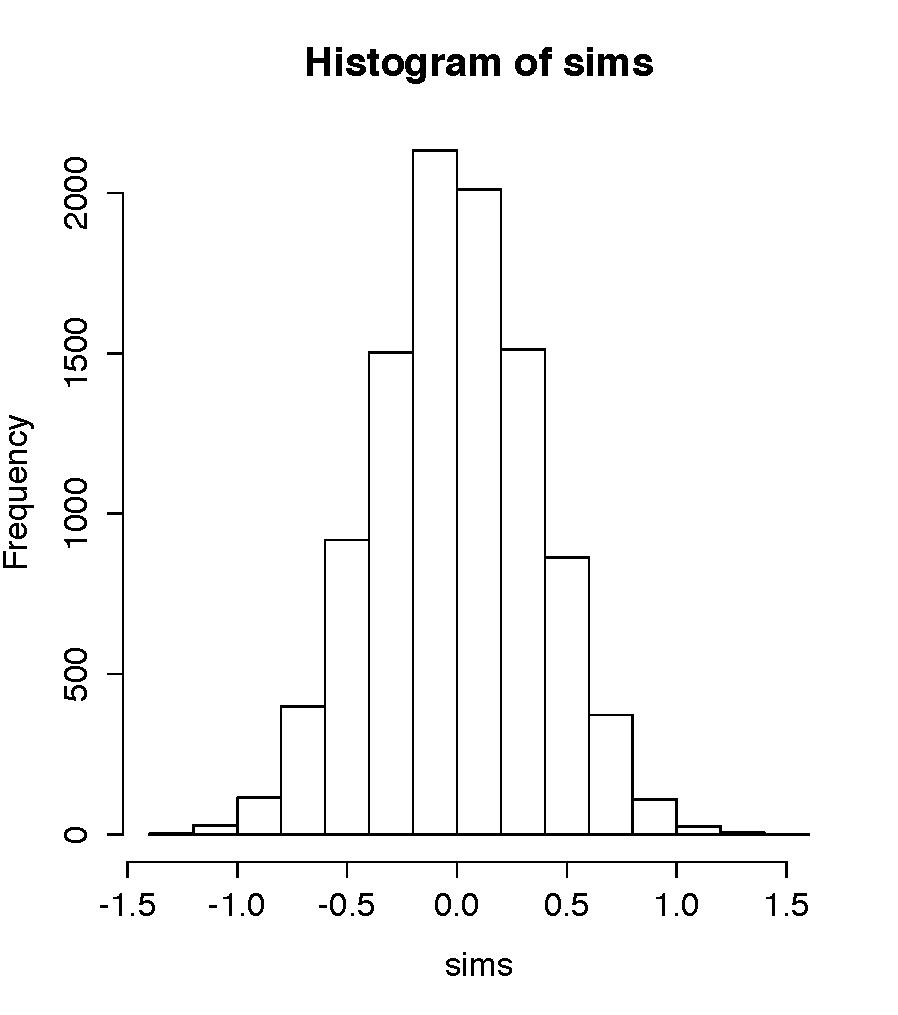
\includegraphics[scale = 0.75]{hist_median_sims}
\caption{Histogram for Question \ref{question:mediansim}}
\label{fig:hist}
\end{figure}


\question This question concerns the ``Pepsi Challenge'' experiment. The setup is identical to the one we used in class except with five cups of each soda rather than four. The experimental procedure is as follows. We first fill five cups with Pepsi and five with Coke. Then we randomize the order of the cups and allow our expert to taste each. Finally, we ask the expert to identify which five cups contain Coke and record the number of cups that she correctly identifies. The idea is to determine whether our expert can really tell the difference between Coke and Pepsi based on the results of the experiment. This question asks to you formalize the experiment as a statistical hypothesis test. Our test statistic $T$ is the number of Cokes that our expert correctly identified.
	\begin{parts}
		\part[5] What is our null hypothesis, $H_0$, in this experiment?
		\begin{solution}[0.75in]
		The null hypothesis is that our so-called ``expert'' is in fact just guessing: she is simply choosing five cups at random and calling them Cokes.
		\end{solution}
		\part[5] What is our alternative hypothesis, $H_1$, in this experiment?
		\begin{solution}[0.75in]
			Our alternative is that the expert has actual skill in discerning the difference between Coke and Pepsi. This is a one-sided alternative: we'll reject the null if she identifies a sufficient number of Cokes correctly.
		\end{solution}
		\part[5] Under $H_0$ what is the probability that $T=5$?
			\begin{solution}[2in]
				Under the null, our expert is merely choosing randomly, and each possible allocation of five cups to ``Coke'' is equally likely. There are 
				$${10\choose 5} = \frac{10!}{5!5!} = 252$$ 
				ways to choose the cups at random, of which only one is correct. Therefore, the desired probability is $\p(T=5|H_0) = 1/252 \approx 0.004$.
			\end{solution}
		\part[5] Under $H_0$ what is the probability that $T=4$? 
			\begin{solution}[2in]
			Under the null, each of the 252 ways to choose five cups is equally likely. The case $T=4$ corresponds to mis-identifying one Coke. There are 5 ways to choose which Coke is mis-identified as a Pepsi, and 5 ways to choose which Pepsi is mis-identified as a Coke. Hence $\p(T=5|H_0) = 25/252 \approx 0.1$
			\end{solution}
		\part[5] Suppose I wanted to test $H_0$ at the 5\% significance level. What is my decision rule given the alternative you specified?
			\begin{solution}[1in]
			Reject $H_0$ if $T>4$ or equivalently if $T=5$.
			\end{solution}
		\part[5] Suppose our expert identified four Cokes correctly. What is the p-value for our test against the alternative you specified?
			\begin{solution}[1in]
				$\p(T\geq 4|H_0) = 26/252 \approx 0.103$.
			\end{solution}
	\end{parts}


\question Suppose there is a logarithmic relationship between random variables $X$ and $Y$, namely $\ln Y_i = \beta X_i + \epsilon_i$ where $\epsilon_i \sim \mbox{iid} (0,\sigma^2)$ is an unobserved error term. 
	\begin{parts}
		\part[5] Suppose we want to estimate $\beta$ by least squares regression using a random sample of observations $(y_1, x_1),\hdots, (y_n, x_n)$. What optimization problem should we solve?
		\begin{solution}[1in]
			In least squares regression, we minimize the sum of squared vertical deviations (residuals). In other words:
				$$\min_\beta \sum_{i=1}^n \left(\ln{y_i} - \beta x_i\right)^2$$
		\end{solution}
		\part[10] Solve the problem from part (a) to derive an explicit formula for $\widehat{\beta}$. You do not need to check the second order condition.
			\begin{solution}[2.9in]
				We differentiate with respect to $\beta$, and manipulate the first order condition as follows:
					\begin{eqnarray*}
					-2\sum_{i=1}^n \left(\ln{y_i} - \beta x_i\right) x_i&=& 0\\
					\sum_{i=1}^n \left(\ln{y_i} - \beta x_i\right)x_i &=& 0\\
					\sum_{i=1}^n \ln{(y_i)} x_i&=&\beta \sum_{i=1}^n x_i^2
					\end{eqnarray*}
				Hence,
					$$\widehat{\beta} = \frac{\sum_{i=1}^n \ln{(y_i)} x_i}{\sum_{i=1}^n x_i^2}$$
			\end{solution}
	\end{parts}



\begin{table}
\footnotesize
\caption{Regression Results}
\paragraph{Regression 1:}
\begin{verbatim}
lm(formula = midterm2 ~ male)
            coef.est coef.se
(Intercept) 81.82     2.12  
male        -0.22     2.91  
---
n = 70, k = 2
residual sd = 12.17, R-Squared = 0.00
	\end{verbatim}
	\paragraph{Regression 2:}
	\begin{verbatim}
lm(formula = midterm2 ~ midterm1)
            coef.est coef.se
(Intercept) 34.63     9.32  
midterm1     0.59     0.12  
---
n = 70, k = 2
residual sd = 10.35, R-Squared = 0.28
	\end{verbatim}
	\paragraph{Regression 3:}
	\begin{verbatim}
lm(formula = midterm2 ~ male + midterm1)
            coef.est coef.se
(Intercept) 34.79     9.47  
male        -0.31     2.50  
midterm1     0.59     0.12  
---
n = 70, k = 3
residual sd = 10.43, R-Squared = 0.28
	\end{verbatim}
	\paragraph{Regression 4:}
	\begin{verbatim}
lm(formula = midterm2 ~ male + male:midterm1 + midterm1)
              coef.est coef.se
(Intercept)   19.31    14.22  
male          26.76    18.82  
midterm1       0.78     0.18  
male:midterm1 -0.34     0.23  
---
n = 70, k = 4
residual sd = 10.34, R-Squared = 0.30
	\end{verbatim}
	\label{tab:reg}
\end{table}


\question This question is based on an dataset containing observations on students in Econ 103: \texttt{male} takes the value 1 if a given student is male, zero otherwise; \texttt{midterm2} gives that student's score on the second midterm; and \texttt{midterm1} gives the student's score on the first midterm. Using this dataset, I estimated four regression models using R. The results appear in Table \ref{tab:reg}. 

\begin{parts}
	\part[5] Suppose I wanted to test the null hypothesis that men and women do just as well, on average, on the second midterm of Econ 103 against the two-sided alternative using a 5\% significance level. I can carry out this test directly from the results present above. Which results should I use and how should I carry out the test? In particular, what is the appropriate test statistic, what is the appropriate critical value, and what is the outcome of the test? 
		\begin{solution}[2.9in]
			We should use the results of the first regression: the coefficient estimate for \texttt{male} is the difference of mean test scores between men and women (i.e. $\bar{x}_M - \bar{x}_W$). The test statistic is the absolute value of the ratio of this estimated coefficient divided by its estimated standard error: $|-0.22/2.91|\approx 0.08$. The approximate critical value for this test is 2, so we fail to reject the null hypothesis.
		\end{solution}
	\part[5] Explain the difference between the models used in Regression 2, versus 3 and 4. Do not comment on the results, only the \emph{models themselves}.
		\begin{solution}[2.9in]
			Regression 2 estimates the same relationship between score on the first midterm and the second for men and women. Regression 3 allows the intercept of the regressions to vary across sex, and Regression 4 allows both the intercept and the slope to vary across sex.
		\end{solution}
	\part[5] Based on the above regression results, what is the sample correlation between students' scores on the two midterms?
		\begin{solution}[2.2in]
			For a simple linear regression, the $R^2$ is the square of the sample correlation between $x$ and $y$. Hence, $\sqrt{0.28}\approx 0.53$ is the sample correlation between scores on the first and second midterm.
		\end{solution}
	\part[5] Explain the meaning of the coefficient estimate \texttt{midterm1} in Regression 2 and construct a 95\% confidence interval for this parameter. What would you conclude on the basis of this interval? 
		\begin{solution}[2.2in]
			This estimate tells us the difference in score on midterm two that we would predict between two groups of students who differed by one point in their scores on midterm one: people who did one point better on the first exam do about 0.6 points better on the second exam. An approximate 95\% confidence for this parameter is $0.6 \pm 0.24$, in other words $(0.36, 0.84)$. This interval does not include zero and is bounded substantially away from it. Our data strongly suggest that people who did better on the first exam continue to do better on the second.
		\end{solution}
	\part[5] Instead of constructing a confidence interval, suppose I wanted to test the null hypothesis that the coefficient on \texttt{midterm1} in Regression 2 is zero against the two-sided alternative. What is my test statistic? Would I reject the null at the 5\% level? What R command should I enter to find the p-value for this test?
		\begin{solution}[2.2in]
			We know immediately that we can reject at the 5\% level since zero is not contained in the confidence interval from part (d). The estimate is about $0.6$ and the standard error is $0.12$ so the test statistic is approximately $5$. To calculate the p-value for the two-sided alternative, we use \texttt{2 * (1 - pnorm(5))}.
		\end{solution}
	\part[10] Suppose we want to predict a student's score on the second midterm. Based on the results given above, do you think we should take into account that student's sex? If so, how should we use this information? Explain your reasoning.
		\begin{solution}
			Based on the above results, it does not seem that a student's sex is helpful in predicting his or her score on the second midterm. In part (a), for example, we found no evidence that men and women score differently on average on the second midterm, using the results of Regression 1. In Regression 3 a 95\% confidence interval for \texttt{male} is approximately $-0.3 \pm 5$, so we find no evidence that we should allow a different intercept for men and women. In Regression 4, a 95\% confidence interval for \texttt{male} is about $27 \pm 38$ while a 95\% confidence interval for \texttt{male:midterm1} is about $-0.34 \pm 46$ so we find no strong evidence that we need to allow a different intercept \emph{or} slope for men versus women. Viewed from a predictive perspective, although the residual standard deviation is lowest in Regression 4,  the difference between this and the value for Regression 2, which does not even consider sex, is minuscule: 0.01 points. 
			\end{solution}
\end{parts}

\end{questions}

\end{document}